\documentclass[11pt]{article}
 
\usepackage{amsmath,amsthm,amssymb,float,tabularx}
\usepackage{graphicx}
\usepackage{latexsym}
 
 
\headheight 10pt
\headsep 20pt
\topmargin 20pt
\oddsidemargin 0pt
\textwidth 170.0mm
\textheight 210.0mm
\pagestyle{myheadings}
\renewcommand{\baselinestretch}{1.25}
\renewcommand{\topfraction}{1}
\renewcommand{\bottomfraction}{1}
\renewcommand{\textfraction}{0}
\setcounter{secnumdepth}{4}
\setcounter{tocdepth}{4}
 
\begin{document}
\tableofcontents
\scriptsize{
\begin{table}[htb!]
\begin{center}
\begin{tabular}{| l | l | l | l | l | l | l |} \hline
gap & minLength	& blockSize & \% & \# correct & \# incorrect & \# missing \\ \hline
2 & 3 & 4 & 5 & 6 & 7 & 8 \\
2 & 3 & 4 & 5 & 6 & 7 & 8 \\ \hline
\end{tabular}
\end{center}
\caption{This is caption}
\label{tbl-fig}
\end{table} 
}

\begin{figure}[htb!]
\begin{center}
\begin{tabular}{c c}
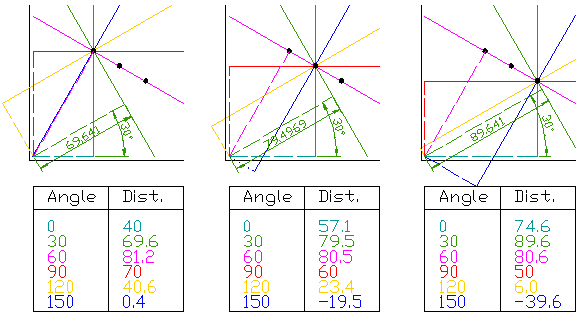
\includegraphics[width=3.0in]{SHT-example2.png} &
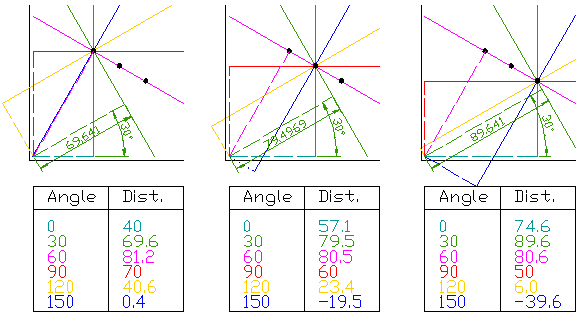
\includegraphics[width=3.0in]{SHT-example2.png} \\
(a) & (b) \\ 
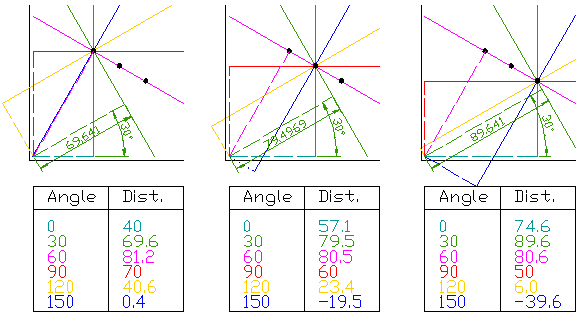
\includegraphics[width=3.0in]{SHT-example2.png} &
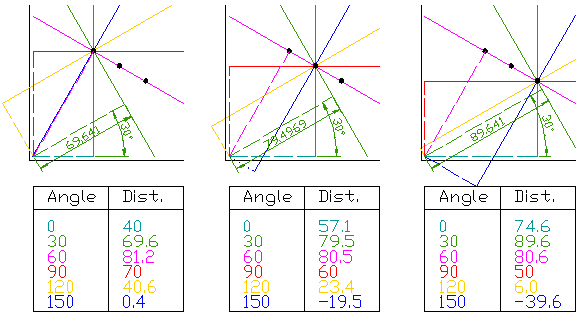
\includegraphics[width=3.0in]{SHT-example2.png} \\
(c) & (d) 
\end{tabular}
\end{center}
\caption{This is an example figure.}
\label{fig1}
\end{figure}

In Figure \ref{fig1}
\end{document}



